\documentclass[a4paper,12pt]{article} 
 
 
%\usepackage[a4paper,vmargin={0mm,10mm},hmargin={10mm,10mm}, includehead,% includefoot]{geometry} \usepackage{fancybox} 
\usepackage{ragged2e} 
\justifying 
\usepackage[T1]{fontenc} 
\usepackage[utf8]{inputenc} 
\usepackage{graphicx} 
\usepackage[russian]{babel}  
\usepackage{geometry} 
 
 
 
 
\geometry{total={210mm,297mm},left=25mm,right=25mm,bindingoffset=0mm, top=20mm,bottom=20mm} 
 
 
 
 
\usepackage{fancyhdr} 
%\pagestyle{fancy} 
\cfoot{Стр. \thepage} 
 
 
\makeatletter 
\renewcommand{\@listI}{% 
\topsep=0pt } 
\makeatother 
 
 
\makeatletter 
\let\old@itemize=\itemize 
\def\itemize{\old@itemize 
\setlength{\itemsep}{0pt} 
\setlength{\parskip}{0pt} 
\setlength{\leftskip}{0pt} 
} 
\makeatother 
 
 
\makeatletter 
\let\old@enumerate=\enumerate 
\def\enumerate{\old@enumerate 
\setlength{\itemsep}{0pt} 
\setlength{\parskip}{0pt} 
\setlength{\leftskip}{0pt} 
}\makeatother 
 
 
\begin{document} 
 
 
%\fancypage{\setlength{\fboxsep}{0pt}\fbox}{} 
 
 
\begin{titlepage} 
\newpage 
 
 
\begin{center} 
\end{center} 
 
 
\vspace{40ex} 
 
 
\begin{center} 
\LARGE РУКОВОДСТВО 
\end{center} 
 
 
\begin{center} 
\Large По работе с приложением ScopeViewer 
\end{center} 
 
 
\vspace{55ex} 
 
 
\begin{center} 
\Large Санкт-Петербург 
\end{center} 
 
 
\begin{center} 
\Large 2017 
\end{center} 
 
 
\end{titlepage} 
 
 
\section*{\hspace{.5cm}Общие сведения } 
\hspace{.5cm}Приложение ScopeViewer предназначено для отображения осциллограмм, записанных в формате COMTRADE (*.cfg) и TEXT FILE (*.txt). В приложение можно выделить четыре основные области:  
\begin{enumerate} 
\item - Панель инструментов. 
\item - Меню осциллограмм. 
\item - Панель дополнительных инструментов. 
\item - График осциллограммы. 
\end {enumerate} 
 
 
\begin{figure}[h] 
\centering 
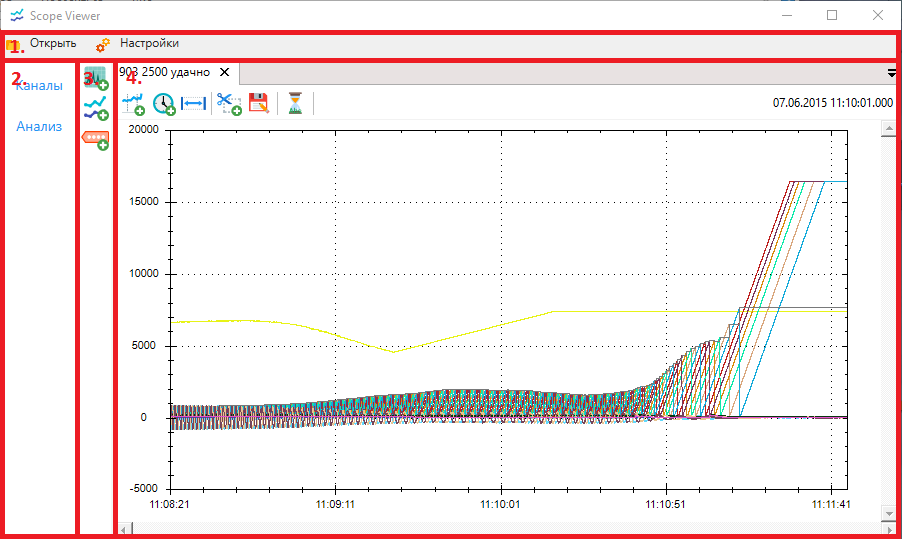
\includegraphics[width=80ex]{image/Screenshot_7.png} 
\caption{Главное окно приложения.} 
\end{figure} 
 
 
\section*{\hspace{.5cm}Панель инструментов } 
\hspace{.5cm}В верхней части окна расположена панель инструментов, на которой размещены кнопки «Открыть» и «Настройки», позволяющие открыть файл осциллограммы и настроить параметры приложения. 
\subsubsection*{\hspace{.5cm} Открыть осциллограмму} 
\hspace{.5cm} При открытии осциллограммы (кнопка «Открыть» 
\includegraphics[width=4ex]{image/OpenFolder.png}) раскрывается окно выбора файлов. 
\subsubsection*{\hspace{.5cm} Настройки приложения} 
\hspace{.5cm} В настройках приложения (кнопка «Настройки» 
\includegraphics[width=4ex]{image/Services-48.png}) можно настроить параметры отображаемых графиков.  
Низкий уровень детализации позволяет увеличить скорость отрисовки, но при этом теряется его качество. Различие между вариантами детализации заключается в количестве отрисовываемых точек для видимой части каждого из каналов. Возможны следующие варианты детализации: низкий (150 точек на канал), средний (400 точек на канал), высокий (1000 точек на канал), очень высокий (10000 точек на канал) и полный (все точки).  
Линии сетки упрощают ориентирование на графике. Можно настроить отображение как основных, так и промежуточных (вспомогательных) линий сетки. Можно выбрать следующий вид: пунктирный, точечный и сплошная линия (для основных линий сетки). Так же можно включить и отключить видимость линии.  
Легенда помогает разобраться в представленных данных. Можно настроить ее отображение, размер и положение на графике. 
\begin{figure}[h] 
\centering 
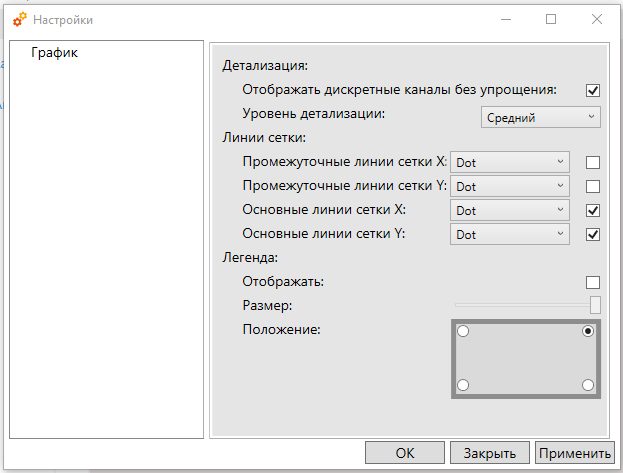
\includegraphics[width=65ex]{image/Screenshot_5.png} 
\caption{Настройки приложения.} 
\end{figure} 
 
 
\section*{\hspace{.5cm} Меню осциллограмм } 
\hspace{.5cm} В меню осциллограммы расположены кнопки «Каналы» и «Анализ», дающие возможность настроить параметры каналов осциллограмм и просмотреть мгновенные значения.  
 
 
\subsubsection*{\hspace{.5cm} Настройка каналов } 
\hspace{.5cm}При открытие меню «Настройка каналов» (кнопка «Каналы» ), отобразятся настройки каналов открытых осциллограмм. Чтобы увидеть подробную информацию о канале необходимо нажать по его названию. Ниже приведены параметры, которые можно изменить в меню настройки каналов: 
\begin{enumerate} 
\item - Выбор типа канала. Предусмотрено два типа каналов: аналоговый и цифровой. Аналоговый подходит для аналоговых величин, а цифровой для отображения дискретных величин. Цифровой канал будет отображаться без упрощения, если в настройках включено отображение дискретного канала без упрощения. Выбрав цифровой канал его можно рассмотреть по битам.  
\item - Выбор типа линии отображаемого канала: сплошная, пунктирная, точечная. 
\item - Выбор типа дискретизации линии отображаемого канала. Возможны следующие варианты: без дискретизации, в начале фронта (ступенчатая и сегментная) и в конце фронта (ступенчатая и сегментная). 
\item - Отобразить или скрыть все каналы осциллограммы на графике. 
\item - Выбрать все каналы осциллограммы. Выбор каналов полезен для создания новой осциллограммы, объединения или для подробного рассмотрения цифрового канала (см. «Панель дополнительных инструментов»). 
\item - Закрыть осциллограмму. 
\item - Включить или отключить отображение канала на графике.  
\item - Выбрать канал. Выбор каналов полезен для создания новой осциллограммы, объединения или для подробного рассмотрения цифрового канала (см. «Панель дополнительных инструментов»). 
\item - Изменить на графике цвет линии отображаемого канала. Нажав на цвет можно выбрать цвет, которым будет отображается линия канала на графике. 
\item - Включить или отключить сглаживание линии канала на графике. 
\item - Отображать канал на графике толстой линией. 
\end {enumerate} 
 
 
\begin{figure}[h] 
\centering 
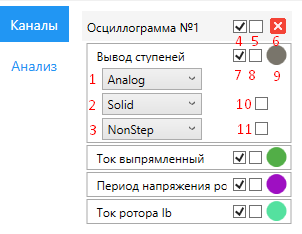
\includegraphics[width=40ex]{image/Channel.png} 
\caption{Настройка каналов.} 
\end{figure} 
 
 
\subsubsection*{\hspace{.5cm} Результаты анализа } 
\hspace{.5cm} Открыть меню «Результаты анализа» (кнопка «Анализ» ) можно только тогда, когда на графике осциллограммы добавлены курсоры.  
В меню «Результаты анализа» отображаются положения курсоров и мгновенные значения каналов в этих положениях. 
 
 
\begin{figure}[h] 
\centering 
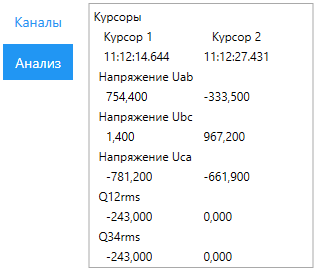
\includegraphics[width=40ex]{image/Screenshot_8.png} 
\caption{Результаты анализа.} 
\end{figure} 
 
 
 
 
 
 
\section*{\hspace{.5cm} Панель дополнительных инструментов} 
\hspace{.5cm}Между областями «Меню осциллограмм» и «График осциллограммы» расположена панель дополнительных инструментов,  позволяющая: добавить новый график, объединить осциллограммы и открыть дискретный канал. 
 
 
Инструмент «Добавить новый график» 
\includegraphics[width=4ex]{image/Chromatography.png} позволяет создать новую осциллограмму. Для этого необходимо выбрать интересующие каналы в меню «Каналы».  
 
 
Инструмент «Объединить осциллограммы» 
\includegraphics[width=4ex]{image/Line_Chart.png} позволяет объединить каналы различных осциллограмм в одну, при условии что они следуют друг за другом. Для этого необходимо в меню «Каналы» выбрать интересующие каналы в осциллограммах.  
 
 
Инструмент «Открыть дискретный канал» 
\includegraphics[width=4ex]{image/Dig_Add.png} позволяет раскрыть канал по битам, при этом тип рассматриваемого канала должен быть дискретный. Одновременно можно рассматривать только один дискретный канал. При открытии будет предложено выбрать дискретность канала. 
 
 
\begin{figure}[h] 
\centering 
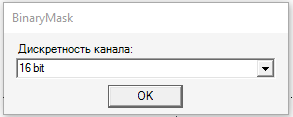
\includegraphics[width=40ex]{image/BinaryMask.png} 
\caption{Дискретность канала.} 
\end{figure} 
 
 
На график осциллограммы добавится цифровой канал, на котором будут отображены следующие линии: линия переходов (темно синяя) «main» (на ней отображены моменты изменения значений в канале) и линии состояния битов (отображают значение того или иного бита). 
 
 
\begin{figure}[h] 
\centering 
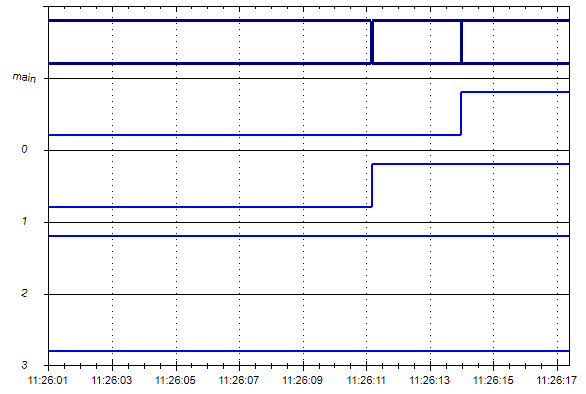
\includegraphics[width=70ex]{image/Screenshot_10.png} 
\caption{Цифровой канал.} 
\end{figure} 
 
 
 
 
\section*{\hspace{.5cm} График осциллограммы} 
\hspace{.5cm}Каждый график осциллограммы открывается в своей вкладке и имеет собственную панель инструментов. В верхнем правом углу отображается штамп времени.  
 
 
\begin{figure}[h] 
\centering 
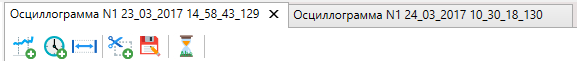
\includegraphics[width=60ex]{image/Screenshot_2.png} 
\caption{Вкладки графиков осциллограмм.} 
\end{figure} 
\paragraph*{\hspace{.5cm} Основные инструменты панели:} 
\begin{enumerate} 
\item 
\includegraphics[width=4ex]{image/Stocks_Add.png} - Добавить курсоры . Для перемещения курсоров нужно нажать по нему и отпустить, после этого его можно свободно перемещать. Курсоры отображаются вертикальными сплошными линиями (красной и синей). В меню «Анализ» будут отображаться мгновенные значения каналов в положениях курсоров. Для удаления курсоров нажмите 
\includegraphics[width=4ex]{image/Stocks_Rem.png}. 
\item 
\includegraphics[width=4ex]{image/Watch_Add.png} - Добавить линию штампа времени на график. 
\includegraphics[width=4ex]{image/Watch_Rem.png} - Убрать линию штампа времени. Штамп времени отображается вертикальной штрих-пунктирной зеленой линией.  
\item 
\includegraphics[width=4ex]{image/Width-48.png} - Масштабирование по горизонтали. 

\includegraphics[width=4ex]{image/Height-48.png} - Масштабирование по вертикали.  

\includegraphics[width=4ex]{image/Resize-48.png} - Масштабирование по горизонтали и вертикали.  
\item 
\includegraphics[width=4ex]{image/Cutting_Add.png} - Обрезать участок осциллограммы. На графике появятся область, которая будет сохранена при применение редактирования.  

\includegraphics[width=4ex]{image/Cutting_Remove.png} - Закрыть область редактирование осциллограммы.  

\includegraphics[width=4ex]{image/Cut_Apply.png} - Применить действия. Осциллограмма будет обрезана по области редактирования.  
\item 
\includegraphics[width=4ex]{image/Save_as_48.png} - Сохранить осциллограмму. Осциллограмма сохраняется в формате TEXT FILE (*.txt). Откроется окно, в котором предложат выбрать название сохраняемого файла. 
\item 
\includegraphics[width=4ex]{image/Time_abs.png} - Переключение между абсолютным и относительным временем.  
\end {enumerate} 
\paragraph*{\hspace{.5cm}Дополнительные инструменты панели:} 
 
 
\hspace{.5cm} 
 
 
Дополнительные инструменты панели графика осциллограмм доступны при открытом дискретном канале. Список дополнительных инструментов представлен в следующем списке.  
 
 
\begin{enumerate} 
\item 
\includegraphics[width=4ex]{image/FlipVertical.png}, 
\includegraphics[width=4ex]{image/FlipHorizontal.png} - Расположение. Меняет расположение отображаемых графиков с вертикального на горизонтальное и наоборот. 
\item 
\includegraphics[width=4ex]{image/Dig_Cancel.png} - Убрать дискретный канал. Удаляет дискретный канал с графика. 
\item 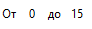
\includegraphics[width=12ex]{image/Screenshot_1.png} - Позволяет редактировать отображение дискретного канала. Указывается диапазон отображаймых битов.
\end {enumerate} 
 
 
Нажав правой кнопкой мыши по вкладкам раскроется меню, в котором можно расположить графики осциллограмм вертикально или горизонтально. При закрытии графика осциллограммы закроется и осциллограмма в меню «Каналы». Так же вкладки можно открепить от области. 
 
 
\begin{figure}[h] 
\centering 
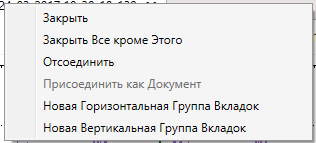
\includegraphics[width=40ex]{image/Screenshot_4.png} 
\caption{Меню вкладки.} 
\end{figure} 
 
 
Нажав правой кнопкой мыши по самому графику откроется меню, в котором можно: копировать график в буфер обмена для последующей вставки в графический файл, сохранить график как рисунок, отправить график на печать, отображать значения точек на графике и управлять масштабом. 
 
 
\begin{figure}[h] 
\centering 
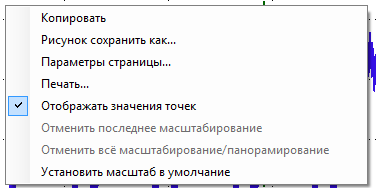
\includegraphics[width=40ex]{image/Screenshot_6.png} 
\caption{Контекстное меню.} 
\end{figure} 
 
 
 
 
 
 
 
 
 
 
\end{document} 
 
 
 
 
 
 
 